\section{SLAM}
When a robot is placed in an unknown environment, it needs to figure out where it is and how the world around it looks. For this SLAM is used, SLAM is short for Simultaneous Localization And Mapping. 
There are multiple SLAM algorithms. In this section, Graph slam and EKF SLAM will be explained.

\subsection{Graph SLAM}
In the perfect world, when a robot moves, it will move exactly as intended. So if a robot is supposed to move 10 in the x direction, the new position will be $x_1 = x_0 + 10$ and $y_1 = y_0$. This is pictured in figure \ref{GraphSLAM01}.
\begin{figure}[h!]
  \caption{A robot in a perfect world, moving 10 in the x direction.}
    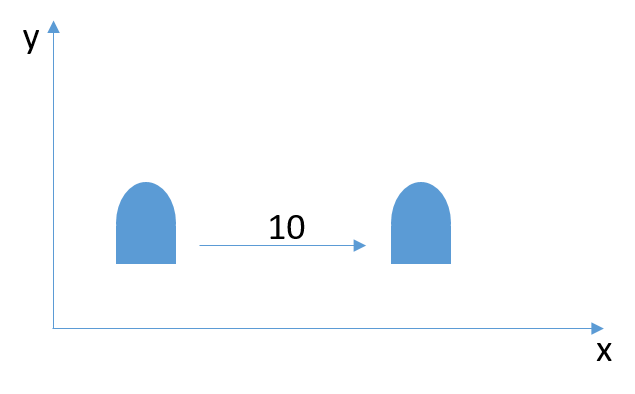
\includegraphics{billeder/GraphSLAM01.png} \label{GraphSLAM01}
\end{figure}

This, however is not the way it actually works. There will always be some motion noise. So instead of hitting the spot perfectly, the robot will hit the spot with some probability, which can be estimated by a Gaussian. So the new robot position will be given by:
\begin{equation}
f(x,y)=\frac{1}{\sqrt{2*\pi*\sigma^2}}*e^(\frac{\frac{1}{2}*(x_1-x_0-10)^2}{\sigma^2}*\frac{1}{\sqrt{2*\pi*\sigma^2}}*e^(\frac{\frac{1}{2}*(y_1-y_0)^2}{\sigma^2}
\end{equation}
This is pictured in figure \ref{GraphSLAM02}.
\begin{figure}[h!]
  \caption{A robot in a non perfect world, moving 10 in the x direction. Noise is estimated as a Gaussian with mean $\mu = [10,0]$ and a standard deviation $\sigma$.}
    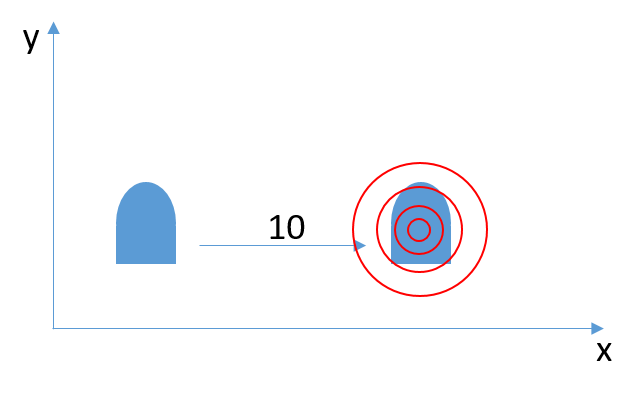
\includegraphics{billeder/GraphSLAM02.png} \label{GraphSLAM02}
\end{figure}


\subsection{EKF SLAM}

%------------------------------------------------